\documentclass[ignorenonframetext,]{beamer}
\PassOptionsToPackage{hyphens}{url}
\usepackage{pgfpages}
\setbeamertemplate{caption}[numbered]
\setbeamertemplate{caption label separator}{: }
\setbeamercolor{caption name}{fg=normal text.fg}
\beamertemplatenavigationsymbolsempty
\usepackage{lmodern}
\usepackage{amssymb,amsmath}
\usepackage{ifxetex,ifluatex}
\usepackage[T1]{fontenc}
\usepackage[utf8]{inputenc}
\usepackage{textcomp} % provides euro and other symbols
\usetheme[]{theme}
\IfFileExists{microtype.sty}{%
\usepackage[]{microtype}
\UseMicrotypeSet[protrusion]{basicmath} % disable protrusion for tt fonts
}{}
%\setlength{\parindent}{0pt}
%\setlength{\parskip}{6pt plus 2pt minus 1pt}
\urlstyle{same}  % don't use monospace font for urls
\makeatletter
\def\maxwidth{\ifdim\Gin@nat@width>\linewidth\linewidth\else\Gin@nat@width\fi}
\def\maxheight{\ifdim\Gin@nat@height>\textheight\textheight\else\Gin@nat@height\fi}
\makeatother
% Scale images if necessary, so that they will not overflow the page
% margins by default, and it is still possible to overwrite the defaults
% using explicit options in \includegraphics[width, height, ...]{}
\setkeys{Gin}{width=\maxwidth,height=\maxheight,keepaspectratio}
% Prevent slide breaks in the middle of a paragraph:
\widowpenalties 1 10000
\raggedbottom
%\setbeamertemplate{section page}{
%\begin{beamercolorbox}[sep=12pt,center]{part title}
%  \usebeamerfont{section title}\insertsection\par
%\end{beamercolorbox}
%}
\setlength{\emergencystretch}{3em}  % prevent overfull lines
\setcounter{secnumdepth}{0}

% set default figure placement to htbp
%\makeatletter
%\def\fps@figure{htbp}
%\makeatother


\title{Les réseaux de neurones}
\author{Fabien Bernier, Elouen Ginat \& Simon Thoby}
\date{Juin 2018}

\begin{document}
\section*{Présentation}
\frame{\titlepage}

\begin{frame}{Sommaire}
\tableofcontents
\end{frame}

\section{Les réseaux de neurones}
\frame{\sectionpage}
\begin{frame}{Structure générale}
	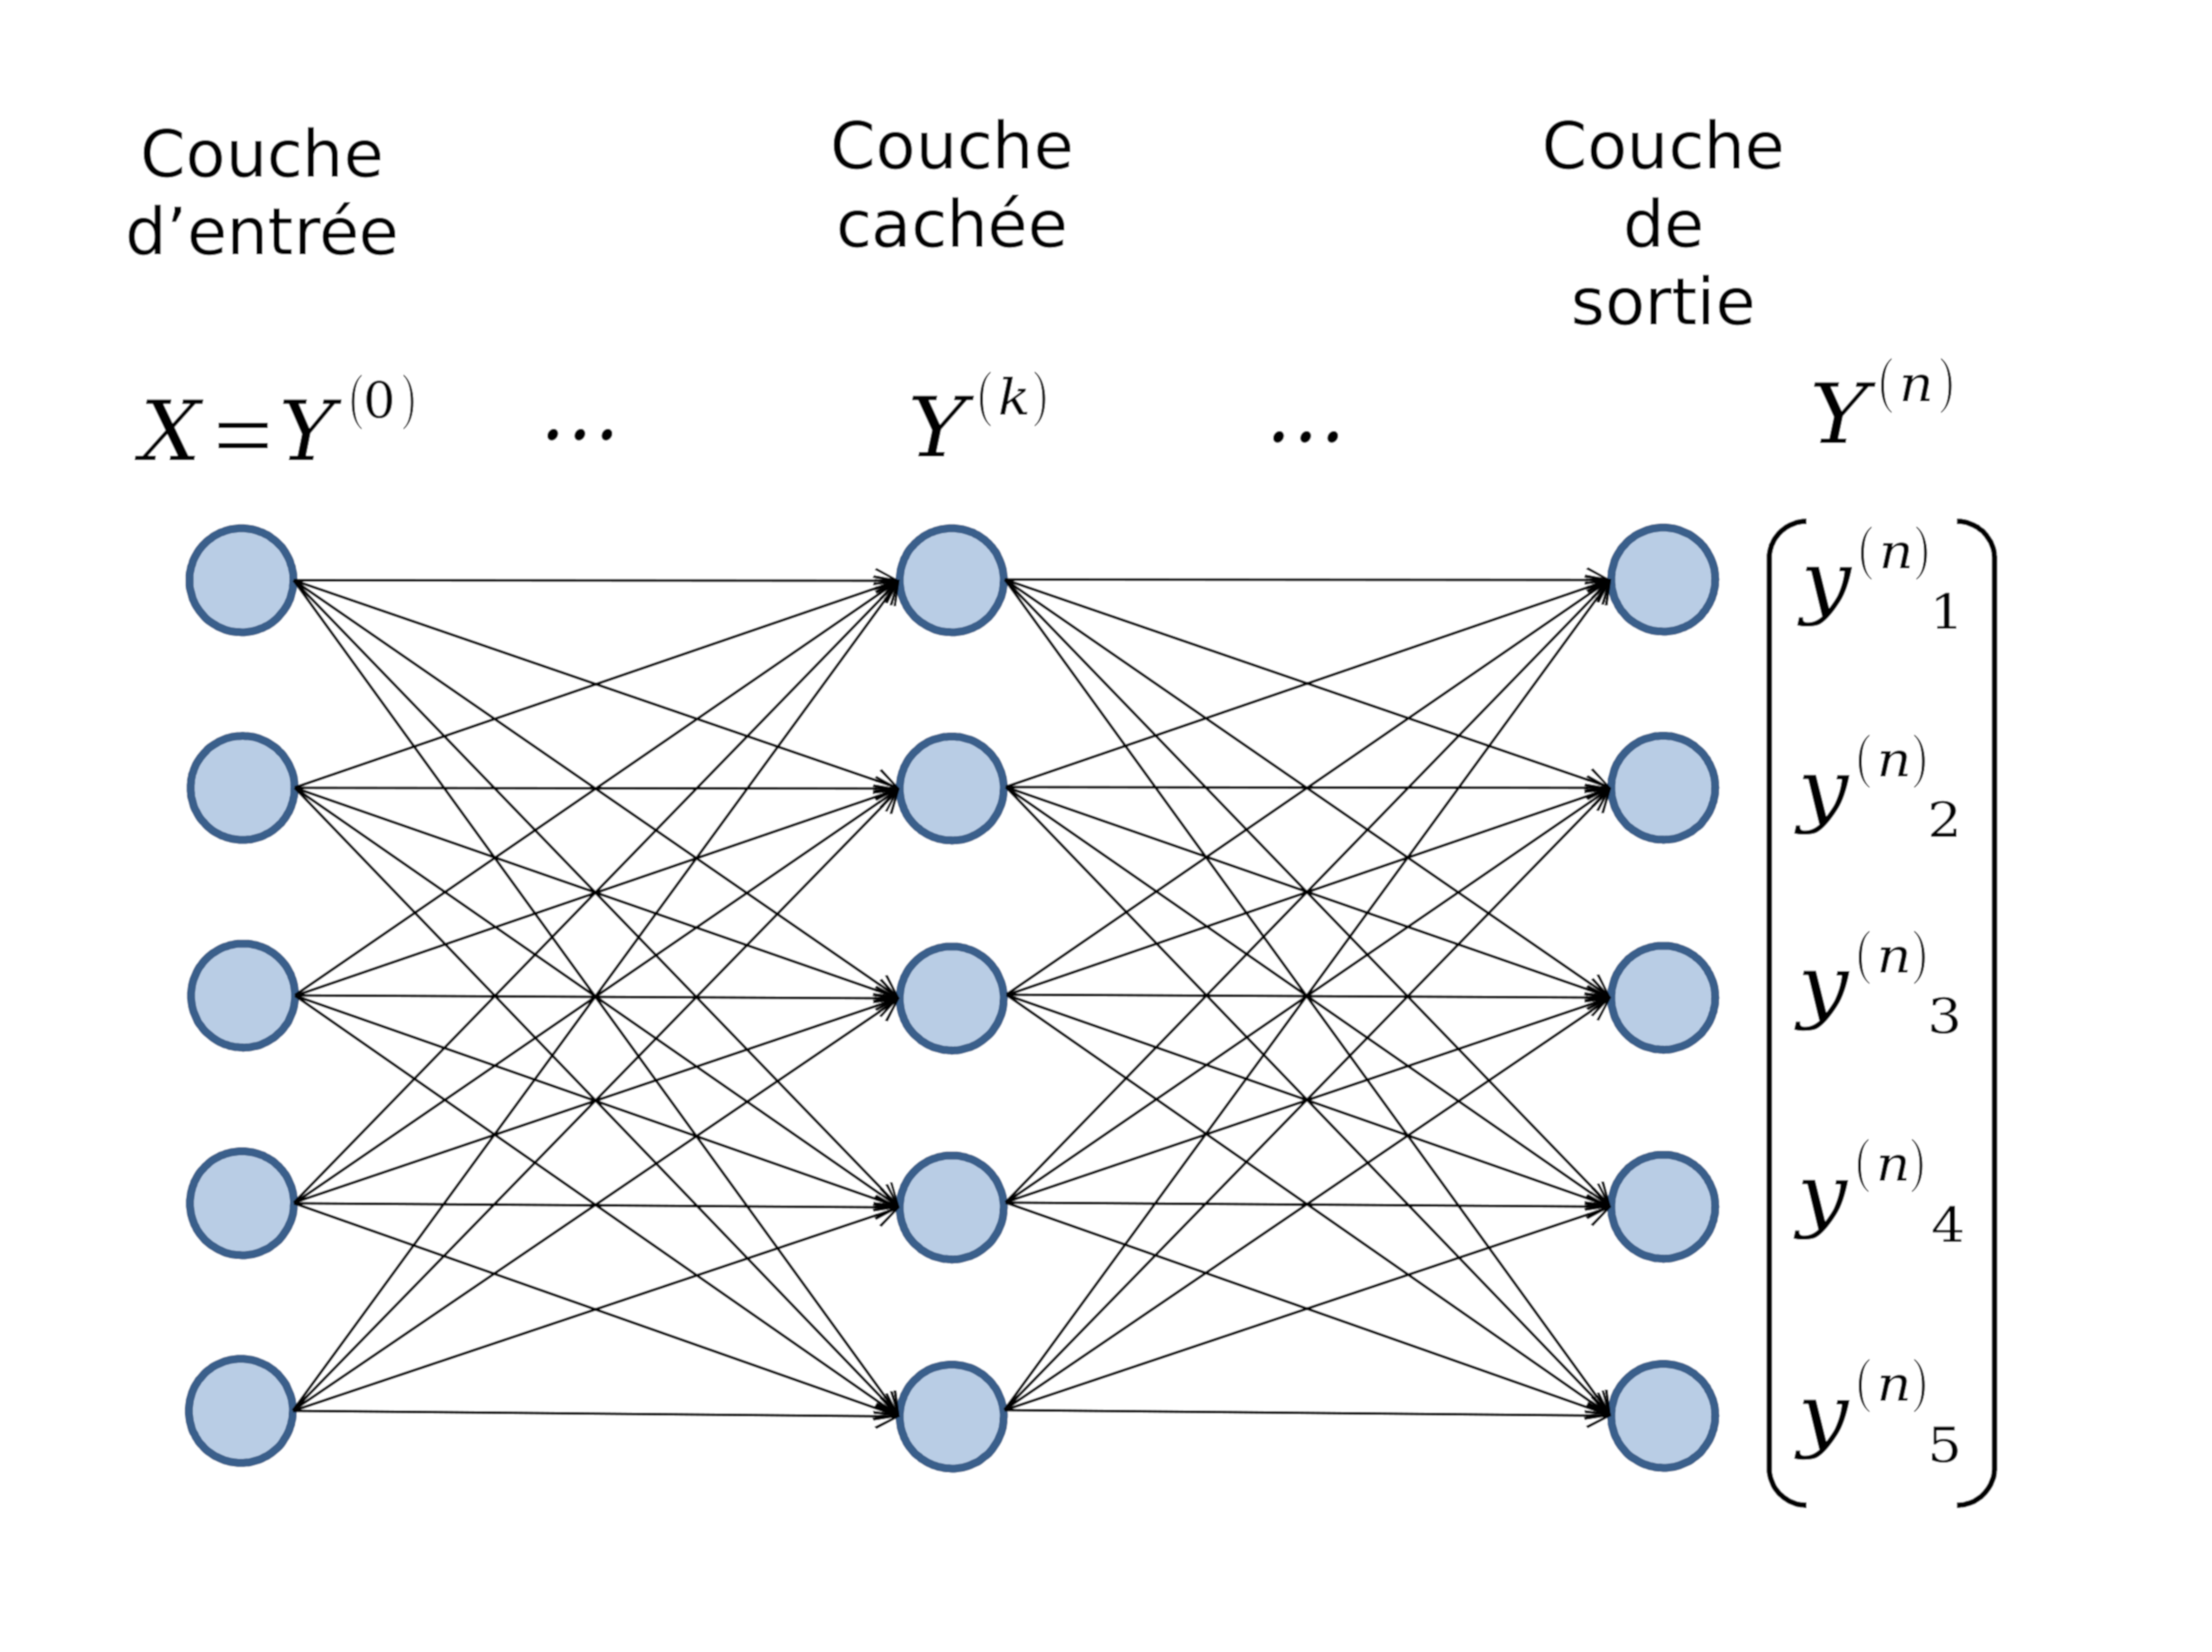
\includegraphics{net-without-train.png}
\end{frame}

\begin{frame}{Fonctionnement du réseau}
	\begin{itemize}
		\item Accepte un vecteur en entrée : que l'on considére comme la première couche, notée $ Y_0 $ \\
		\item Pour chaque couche, on génére un nouveau vecteur à partir de la couche précédente en effectuant une somme pondérée des valeurs de la couche précédente : \[ Y_n = \alpha(W_n . Y_{n-1} + B_n) \]
			Avec :
		\begin{itemize}
			\item $ \alpha $ : une fonction qui sert à améliorer l'efficacité du réseau en normalisant les sorties, classiquement $ \alpha : x \mapsto \frac{1}{1+e^{-x}} $
			\item $ W_n $ : les poids de passage de la couche $ n-1 $ à $ n $
			\item $ B_n $ : les biais de la couche $ n $, qui permettent au réseau d'approximer des fonctions qui ne s'annulent pas quand l'entrée est nulle
		\end{itemize}
		\item Retourne un vecteur en sortie : la sortie de la dernière couche, c'est-à-dire $ Y_n $
	\end{itemize}
\end{frame}

\begin{frame}{Fonctionnement du réseau - suite}
	\begin{itemize}
		\item On dispose pour créer le réseau de deux jeux de données assez conséquent (typiquement plusieurs milliers d'images dans notre cas) : l'un sert à entraîner le réseau et l'autre sert à en tester l'efficacité.
		\item //TODO: schéma			
	\end{itemize}
\end{frame}

\section{La rétropropagation}
\begin{frame}{Approximation d'une fonction}
	À l'instar du théorème d'approximation d'une fonction continue par un polynôme (Stone-Weierstrass), les réseaux de neurones ont pour but d'approximer une fonction (dont on ne connaît généralement pas l'expression) en utilisant l'algorithme dit de «descente du gradient». Le principe est le suivant:
	\begin{itemize}
		\item Le gradient indique la direction de l'augmentation d'une fonction.
		\item On peut donc considérer la fonction $E$ qui indique l'«erreur» du réseau, c'est à dire la distance entre les sorties du réseau et les valeurs attendues en sortie.
		\item Notre but est donc de faire tendre les sorties du réseau vers les valeurs attendues, donc de minimiser cette fonction.
		\item Pour ce faire, on dérive l'erreur par rapport aux paramètres de notre réseau (les poids et les biais) avec une entrée constante (on cherche à réduire l'erreur du réseau sur le vecteur d'entrée, et celui-ci ne varie donc pas au cours de l'exécution de l'agorithme). Puis on mets à jour les poids et les biais:
		\[ w_{ij}^{(n)} \longleftarrow w_{ij}^{(n)} - \eta \frac{\partial{E}}{\partial{w_{ij}^{(n)}}} \]
	\end{itemize}
\end{frame}

\frame{\sectionpage}
\begin{frame}{}

\[ P^{(k)} = W^{(k)}Y^{(k-1)}+B^{(k)}  \]

\[ \alpha : x \mapsto \frac{1}{1+e^{-x}} \]

\[ Y^{(k)} = \tilde\alpha(P^{(k)}) \]

\[ E = \frac{1}{2} \sum_{i=1}^l (y_i^{(n)}-a_i)^2 \]

\end{frame}

\begin{frame}{}

\[ b_i^{(n)} \longleftarrow b_i^{(n)} - \eta \frac{\partial{E}}{\partial{b_i^{(n)}}} \]

\[ w_{ij}^{(n)} \longleftarrow w_{ij}^{(n)} - \eta \frac{\partial{E}}{\partial{w_{ij}^{(n)}}} \]

\[ \frac{\partial{E}}{\partial{b_i^{(n)}}} = \frac{\partial{E}}{\partial{p_i^{(n)}}} \frac{\partial{p_i^{(n)}}}{\partial{b_i^{(n)}}} \]

\[ p_i^{(n)} = \sum_{j=1}^l w_{ij}^{(n)} y_j^{(n-1)} + b_i^{(n)} \]

\end{frame}

\begin{frame}{}

\[ \delta_i^{(n)} = \frac{\partial{E}}{\partial{p_i^{(n)}}} = \frac{\partial{E}}{\partial{b_i^{(n)}}} \]

\[ \delta_i^{(n)} = \frac{\partial{E}}{\partial{p_i^{(n)}}} = \frac{\partial{E}}{\partial{y_i^{(n)}}} \frac{\partial{y_i^{(n)}}}{\partial{p_i^{(n)}}} \]

\[ y_i^{(n)} = \alpha(p_i^{(n)}) \implies \frac{\partial{y_i^{(n)}}}{\partial{p_i^{(n)}}} = \alpha'(p_i^{(n)}) \]

\[ E = \frac{1}{2} \sum_{i=1}^l (y_i^{(n)}-a_i)^2 \implies \frac{\partial{E}}{\partial{y_i^{(n)}}} = y_i^{(n)} - a_i \]

\end{frame}

\begin{frame}{}

\[ \delta_i^{(n)} = \alpha'(p_i^{(n)}) (y_i^{(n)} - a_i) \]

\[ \frac{\partial{E}}{\partial{w_{ij}^{(n)}}} = \frac{\partial{E}}{\partial{p_i^{(n)}}} \frac{\partial{p_i^{(n)}}}{\partial{w_{ij}^{(n)}}} \]

\[ p_i^{(n)} = \sum_{j=1}^l w_{ij}^{(n)} y_j^{(n-1)} + b_i^{(n)} \implies \frac{\partial{E}}{\partial{w_{ij}^{(n)}}} = y_j^{(n-1)} \]

\[ \frac{\partial{E}}{\partial{p_i^{(n)}}} = \delta_i^{(n)} = \alpha'(p_i^{(n)}) (y_i^{(n)} - a_i) \]

\[ \frac{\partial{E}}{\partial{w_{ij}^{(n)}}} = \alpha'(p_i^{(n)}) (y_i^{(n)} - a_i) y_j^{(n-1)} \]

\end{frame}

\section{Localisation des villes}
\frame{\sectionpage}
\begin{frame}{Identifier la présence de villes (algorithme à seuil)}
%\includegraphics{principe-convolution.png}
%\includegraphics{image-exemple.png}
%\includegraphics{convolution-exemple.png}
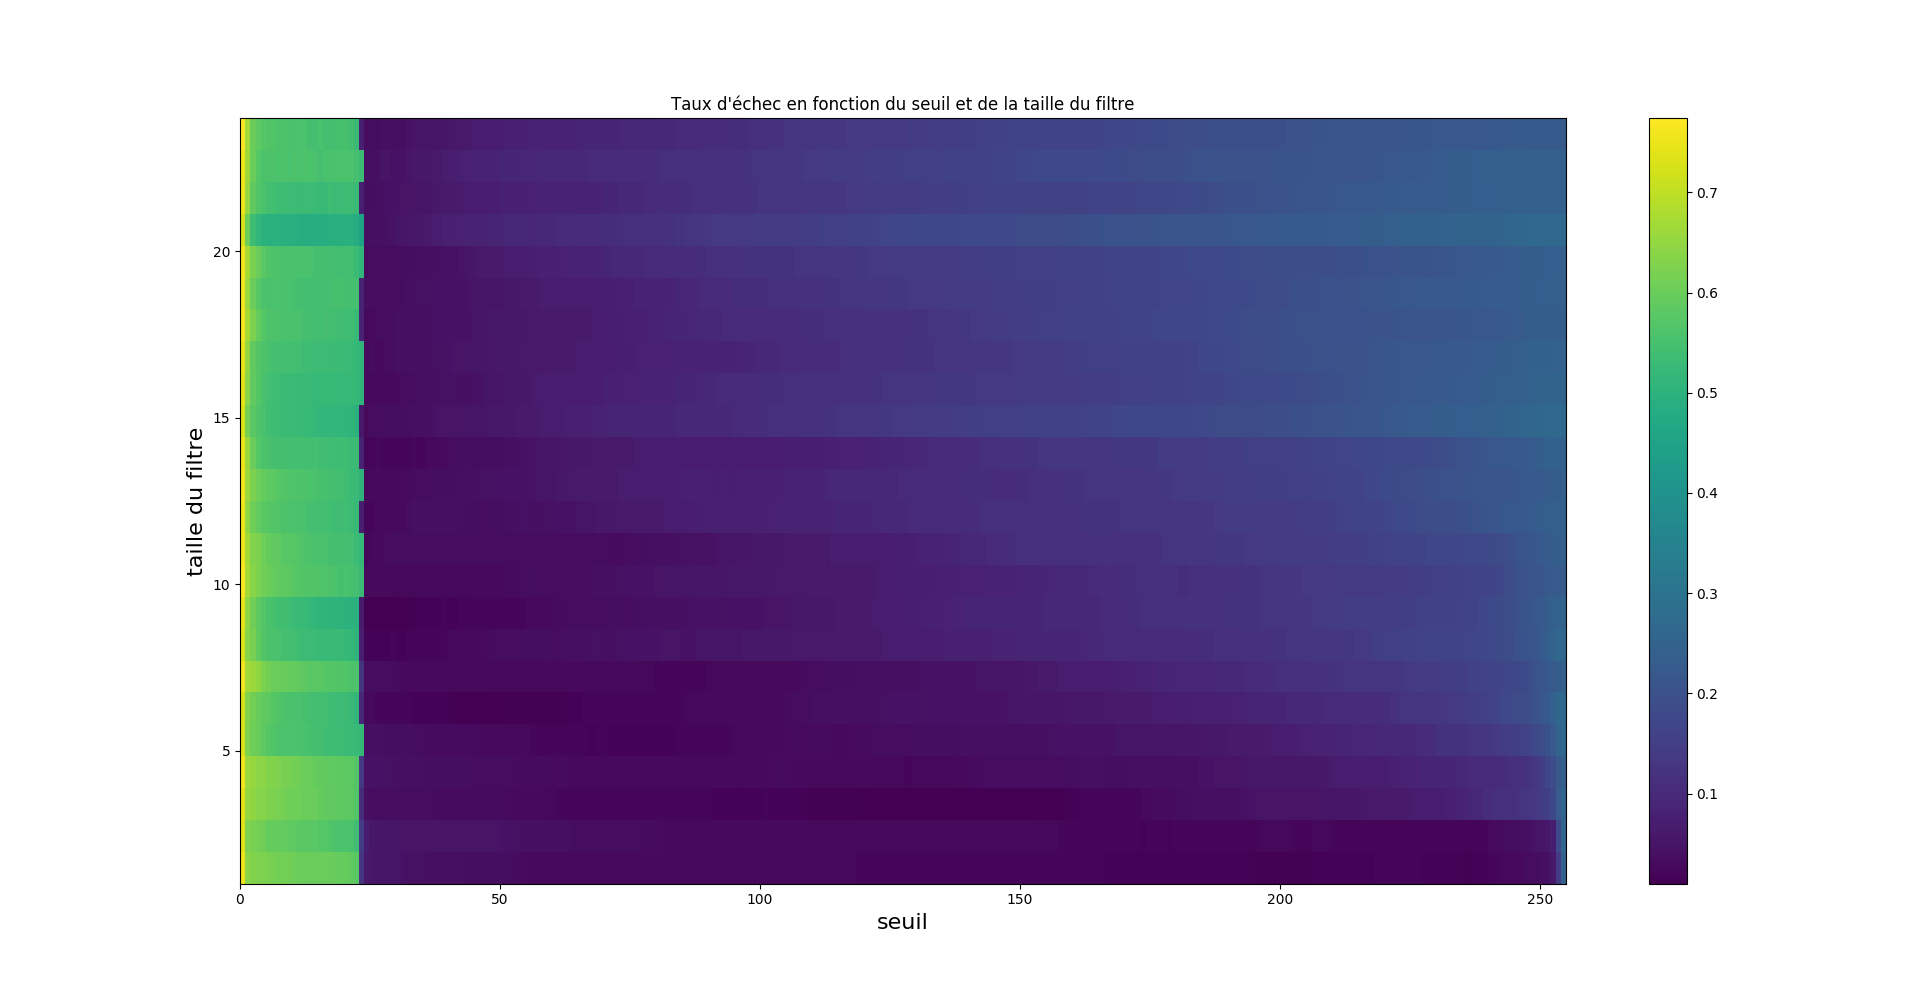
\includegraphics{filtre_vs_seuil.png}
\end{frame}


\end{document}
